\documentclass[11pt]{article}
\usepackage[utf8]{inputenc}
\usepackage[T1]{fontenc}
\usepackage[brazil]{babel}
\usepackage{newtxtext} % Times New Roman
\usepackage[top=3cm, bottom=2cm, left=3cm, right=2cm]{geometry}
\usepackage{ragged2e}
\usepackage{enumitem}
\usepackage{setspace}
\usepackage{makeidx}
\usepackage{graphicx}
\usepackage{afterpage}
\usepackage{booktabs}
\usepackage{float}
\usepackage{tikz}
\usetikzlibrary{fit,shapes.geometric}
\makeindex % Criar índice depois

\newcounter{nodemarkers}
\newcommand\circletext[1]{%
    \tikz[overlay,remember picture] 
        \node (marker-\arabic{nodemarkers}-a) at (0,1.5ex) {};%
    #1%
    \tikz[overlay,remember picture]
        \node (marker-\arabic{nodemarkers}-b) at (0,0){};%
    \tikz[overlay,remember picture,inner sep=2pt]
        \node[draw,ellipse,fit=(marker-\arabic{nodemarkers}-a.center) (marker-\arabic{nodemarkers}-b.center)] {};%
    \stepcounter{nodemarkers}%
}

% Início do corpo do texto
\begin{document}

\justifying % Texto justificado
\onehalfspacing % Espaçamento de 1,5 linha
\setlength{\parindent}{0cm}  % Indentação dos parágrafos
\renewcommand*\familydefault{\rmdefault}
%-----------------------------------------------------------%
% Capa                                
%-----------------------------------------------------------%
\thispagestyle{empty}
\begin{center}

\includegraphics[scale=0.6]{capa/logo-dep.jpg}\\
\vspace*{.8cm}
{\huge \textbf{UNIVERSIDADE FEDERAL DE SÃO CARLOS}}\\
\vspace*{.8cm}
{\Larsge \textbf{SIMULAÇÃO DE SISTEMAS}}\\s
\vspace*{3cm}
{\Large \textbf{ANÁLISE DE DADOS HISTÓRICOS DE UM CALL CENTER}}\\
\vspace*{4.5cm}
\begin{flushright}
    \onehalfspacing
    {\Large  Paulo Roberto Mattielo Filho - 792323}\\
    {\Large  Pedro Peverari Di Lallo - 792328}\\
    {\Large  Lucas Gabriel Malheiros - 769837}\\
    {\Large  Vinícius Nobre - }\\
    \vspace*{.3cm}
    {\Large \textbf{Professor:}}
    {\Large VCBC}\\
\end{flushright}
\vspace*{\fill}
{\large \bf SÃO CARLOS / 2023}
\end{center}



\newpage{}
\tableofcontents{}
\newpage{}

\section{Introdução}
\label{section: intro}
\subsection{Descrição do problema}
ESCREVER UMA DESCRIÇÃO (PRA VALER) DO PROBLEMA DO CALL-CENTER E QUAIS QUESTÕES VAMOS ABORDAR.

\subsection{Alterações da versão anterior}
Descrição mais detalhada do problema da central de atendimentos.\\
Os gráficos de linhas das Figuras \ref*{fig: chamados-tempo}, \ref*{fig: t_servico-tempo}, \ref*{fig: espera-tempo} e \ref*{fig: arrivals-tempo} foram substituídos por gráficos de dispersão.\\
A Figura \ref*{fig: correlogram} foi adicionada ao estudo de correlação das variáveis na Seção \ref*{section: correlacao-anual} para auxiliar na visualização do resultado obtido pelo teste de correlação de Spearman.\\
As seções de introdução e conclusão foram reorganizadas para a escrita de novos conteúdos.\\
Realização dos testes de aderência mensais para tempos entre chegadas na Seção \ref*{section: fit-arrivals}.\\
Correção de erros gerais de redação e referências.



\section{Análise de dados}
Na primeira etapa do projeto, foi realizada a modelagem e análise dos dados referentes às ligações recebidas por uma central de atendimentos. Para isso, foram analisadas diferentes variáveis para que seus comportamentos fossem modelados. Sendo assim, o projeto busca sanar os problemas relacionados à eficiência nos sistemas de atendimento, identificando possíveis gargalos.

\begin{figure}[H]
    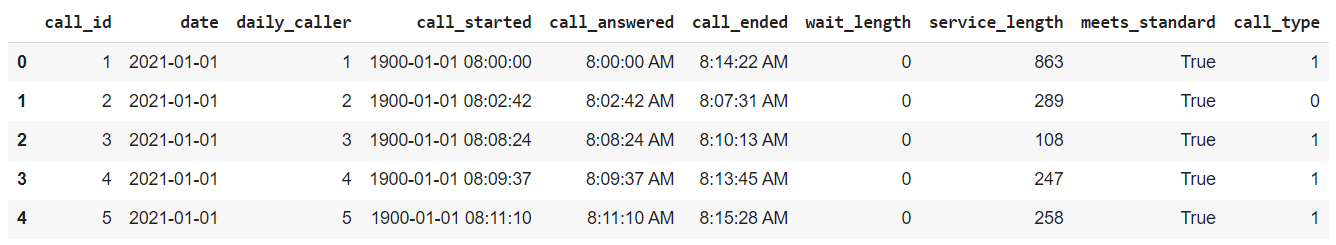
\includegraphics[scale= 0.6]{analise-de-dados/intro-analise/imgintro.png}
    \caption{Banco de dados - 5 primeiras chamadas}
    \label{fig: bd_img}
\end{figure}

Na Figura \ref*{fig: bd_img}, pode-se observar a estrutura da base de dados, assim como as colunas descritas a seguir:

\begin{itemize} 
    \item"call\_id" é a identificação da ligação (chave primária);
    \item"date"\;é a data da ligação;
    \item "daily\_caller"\;numera as ligações em um dia;
    \item"call\_started", "call\_answered" e "call\_ended"\;são os instantes de chegada, atendimento e término  da ligação, respectivamente;
    \item "wait\_length"\;é o tempo de espera;
    \item"service\_length"\;é o tempo de atendimento;
    \item"meets\_standard"\;retorna verdadeiro caso o tempo de espera seja menor do que um minuto;
    \item"call\_type" é o tipo da ligação.
\end{itemize}

Todos os tempos da base de dados estão em segundos.\\
Para os testes de hipóteses atrelados às diferenças entre essas variáveis em diferentes períodos foi utilizado o teste de Kolmogorov-Smirnov para duas amostras, que possui caráter não paramétrico, com as seguintes hipóteses:\\

\begin{center}
$H_0$ : As amostras seguem uma mesma distribuição de probabilidade\\
$H_A$ : As amostras seguem distribuições de probabilidade diferentes
\end{center}

Posteriormente à confirmação positiva da diferença entre amostras, foi realizado o teste de aderência das amostras às distribuições cauchy, chi quadrado, exponencial, gamma, lognormal, normal, powerlaw, rayleigh e uniforme.\\
Por fim, para analisar as correlações entre variáveis, foram realizadas regressões lineares e exponenciais.\\

\subsection{Ferramentas utilizadas}
A modelagem e as análises estatísticas do projeto foram realizadas utilizando a linguagem Python em sua versão 3.9, por meio do ambiente Google Colab.\\
Para isso, foram utilizadas as seguintes bibliotecas de Python:

\begin{itemize}
    \item Jupyter-notebook;
    \item Pandas;
    \item Numpy;
    \item Seaborn;
    \item Fitter;
    \item Scipy;
    \item Tabulate;
    \item Scikit-learn;
    \item Statsmodels;
    \item Matplotlib.
\end{itemize}
\subsection{Análise anual}
Inicialmente, foram levantadas as quantidades de ligações registradas durante o ano e a quantidade total de falhas, assim como o percentual de falhas. No ano de 2021, que contou com 261 dias de trabalho, foram registradas 51.708 ligações, sendo que 4.227 destas demoraram mais de 60 segundos para serem atendidas, caracterizando falha do processo. O percentual destas falhas para o ano foi de 8,17\%, valor que atende as especificações de desempenho da empresa. No entanto, como este valor representa apenas uma média anual, devemos buscar compreender o problema da empresa ao avaliar o comportamento das variáveis relevantes do processo ao longo do ano.

\subsubsection{Quantidade de chamados por dia}
A Figura \ref*{fig: chamados-tempo} apresenta a quantidade de chamadas recebidas por dia ao longo do ano. É possível perceber uma relação de dependência entre a quantidade de ligações recebidas e os dias do ano, visto que o número de chamadas cresce ao longo do ano. Esse comportamento pode ser responsável pelo aumento do percentual de falhas em meses próximos ao fim do ano. Posteriormente, será descrito um estudo de regressão para estes dados.

\begin{figure}[h]
    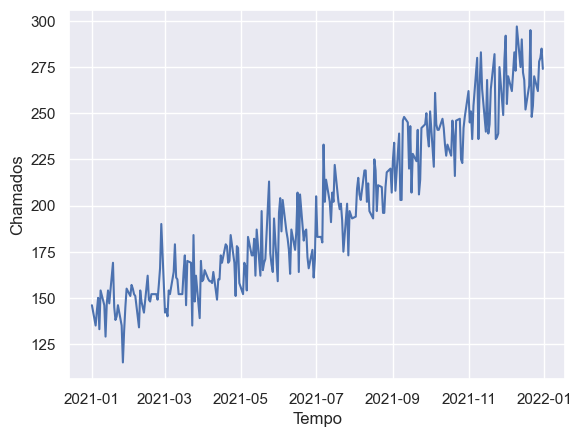
\includegraphics{analise-de-dados/anual/chamados.png}
    \caption{Quantidade de chamadas recebidas ao longo do tempo}
    \label{fig: chamados-tempo}
\end{figure}

\subsubsection{Análise e descrição dos tempos de espera e serviço}
Como os tempos de espera (\textit{wait length}) e serviço (\textit{service length}) já estão calculados, podemos analisar seu comportamento.

\begin{table}
\centering
    \begin{tabular}{lr}
        % \begin{center}
            \toprule
            {} &  Tempo de espera \\
            \midrule
            count &   51708.000  \\
            mean  &      17.035  \\
            std   &      64.061  \\
            min   &       0.000  \\
            25\%   &       0.000  \\
            50\%   &       0.000  \\
            75\%   &       0.000  \\
            max   &     983.000  \\
        % \end{center}
        \bottomrule
        % \label{tab: describe-wait}
    \end{tabular}
\caption{Estatística descritiva dos tempos de espera}
\label{tab: descricao-espera}
\end{table}

Teste

\subsection{Análise mensal}
Foi realizada uma agregação mensal a fim de visualizar as tendências das variáveis do sistema estudado ao longo do ano. Para isso, foi gerada uma tabela com um resumo das médias dos tempos de espera, serviço e de tempo entre chegadas das ligações mês a mês.\\
A partir disso, foi possível calcular a porcentagem de falhas ("\%\_failure") com base na divisão do número total de ligações que demoraram mais de 60 segundos para serem atendidas pelo total de ligações atendidas em cada mês.\\
A partir da Figura \ref*{fig: tmes} é possível visualizar alguns dados relevantes e transformar a base de dados com filtro mês a mês em informações capazes de nos demonstrar o comportamento do processo de atendimento nos quesitos tempo de espera médio, duração média do atendimento, média do tempo entre as chegadas, média do número de ligações recebidas e também a porcentagem de falhas.  

\begin{figure}[H]
    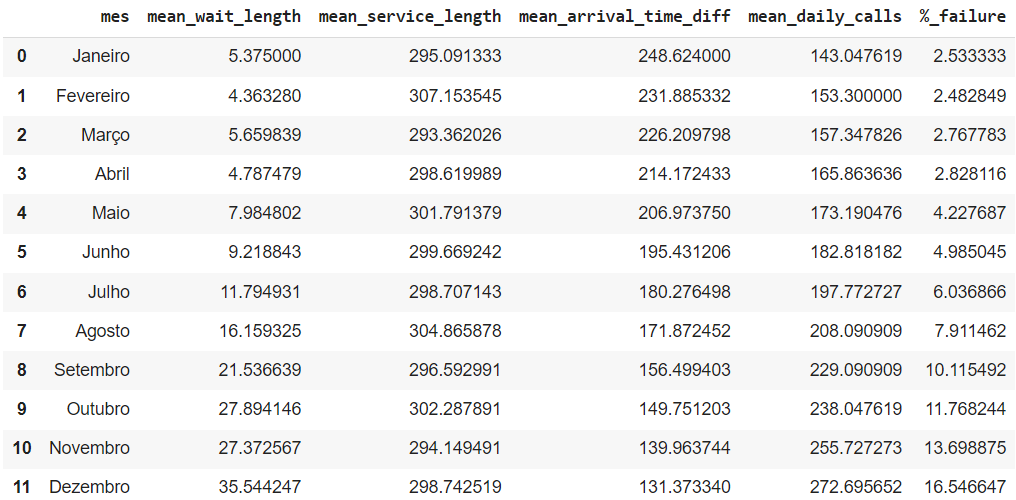
\includegraphics[scale=0.75]{analise-de-dados/mensal/tabmens.png}
    \caption{Tabela de resumo das médias dos tempos de espera, serviço e de chegada de ligações mês a mês}
    \label{fig: tmes}
\end{figure}

Realizando uma análise de cada uma das variáveis do sistema, apoiando-se nos testes de hipótese realizados anteriormente, é possível obter as seguintes conclusões a respeito dessas variáveis:
\begin{itemize}
    \item Tempo de espera: aumenta mês a mês;
    \item Média do tempo de serviço: relativamente constantes;
    \item Tempo entre chegadas: diminui mensalmente;
    \item Número de ligações: aumenta mensalmente;
    \item Percentual de falhas: aumenta mês a mês. A partir de setembro de 2021, a tolerância de 10\% que foi estipulada pelo
     gerente é superada.\\
\end{itemize}

Portanto, o percentual de falhas, aqui definido como o percentual de chamadas que demoram mais de 60 segundos para serem atendidas, aumenta mês a mês, ultrapassando, a partir de setembro de 2021,
a tolerância de 10\% necessária para cumprir a meta de desempenho de 90\% das chamadas atendidas em até 1 minuto.
\subsection{Análise trimestral}
Agregando os valores para períodos trimestrais conseguimos chegar aos dados presentes na Tabela \ref*{fig: tritab_img}:

\begin{figure}[H]
    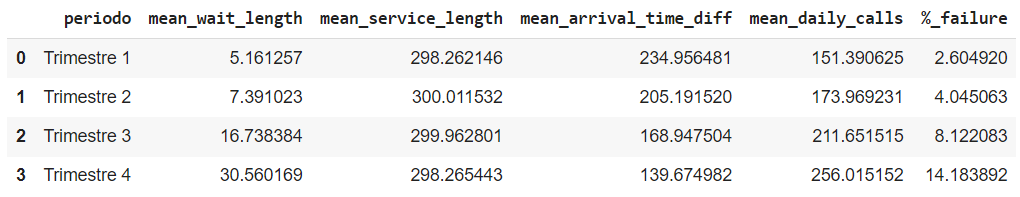
\includegraphics[scale=0.7]{analise-de-dados/trimestral/tritab.png}
    \caption{Tabela de resumo das médias dos tempos de espera, serviço e de chegada de ligações mês a mês}
    \label{fig: tritab_img}
\end{figure}

Tal análise trimestral acaba subestimando a porcentagem de falhas e acaba ocultando algumas informações como a falha no mês de setembro, que está no terceiro trimestre e passa a estar fora da zona de falha estipulada pela gerência.\\
Além disso, também é notável que o caminho correto não é agregar o intervalo de chegadas em períodos ainda maiores, como no trimestre, já que este é um valor alterado mensalmente.\\
Por fim, é possível observar que algumas conclusões semelhantes serão alcançadas em uma análise de cada uma das variáveis, no entanto, há uma perda de informações relevantes, não sendo a melhor maneira de observar o processo.\\
\subsection{Análise semanal}
O ponto principal para a escolha ou não da análise semanal é justamente a existência de diferenças das amostras semanais entre si, que justificaria posterior análise dos dados para melhor compreensão.\\
\subsubsection{Análise dos tempos de espera e serviço}
O teste não paramétrico de Kolgomorov Smirnov novamente foi utilizado para realização do teste de hipótese.\\
Para que não houvesse uma matriz com as respostas desnecessariamente grande (matriz 52x52) foi realizado o teste apenas para as semanas dos meses de dezembro e janeiro.\\
\begin{center}
    \begin{figure}[H]
        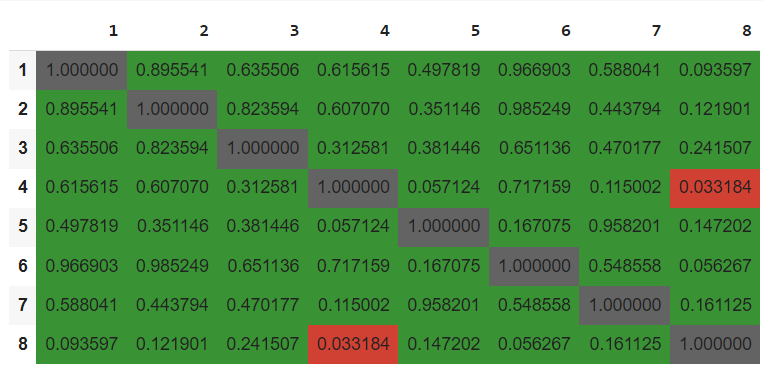
\includegraphics{analise-de-dados/semanal/janas.png}
        \caption{Kolgomorov Smirnov - teste para intervalos de chegada nas semanas de janeiro}
        \label{fig: jan_as_img}
    \end{figure}
    \begin{figure}[H]
        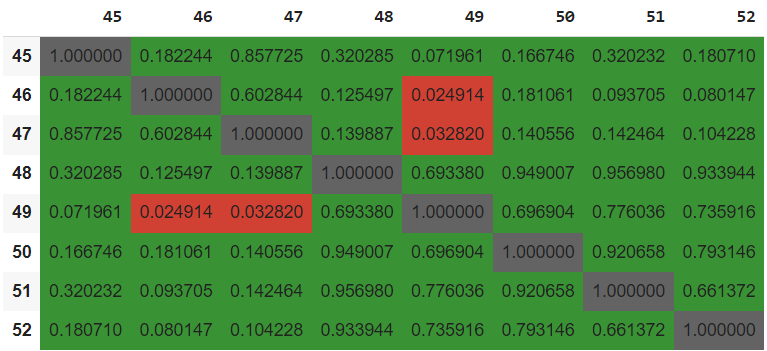
\includegraphics{analise-de-dados/semanal/dezas.png}
        \caption{Kolgomorov Smirnov - teste para intervalos de chegada nas semanas de dezembro}
        \label{fig: dez_as_img}
    \end{figure}
\end{center}
A figura \ref*{fig: jan_as_img} realiza o teste para os tempos de intervalo de chegada no mês de janeiro\\
A figura \ref*{fig: dez_as_img} realiza o teste para os tempos de intervalo de chegada no mês de dezembro\\
Foi possível observar que no horizonte de planejamento semanal, semanas subsequentes tendem a ter intervalos de chegada que seguem a mesma distribuição de probabilidade e, portanto, o planejamento semanal não é interessante para esse problema, visto que não é possível perceber as diferenças de demanda nesse nível de análise.
\subsection{Estudos de Regressão}

Ao montarmos a visualização dos tempos de chegada ao longo do tempo percebemos que havia tendência nos dados. Para isso, primeiro, calculamos todos os tempos de chegada das chamadas, subtraindo o horário de recebimento de uma chamada subsequente pelo da anterior, isto é:

$$Tempo_{chegada}(c_n) = t_n - t_{n-1}$$ 


Depois, as chamadas foram classificadas por dia, e, assim, calculado o tempo de chegada médio diário delas. O principal intuito desta etapa é facilitar a visualização da evolução desse parâmetro ao longo do tempo. O gráfico obtido por essa operação está abaixo, na figura 13.

\begin{figure}[H]
    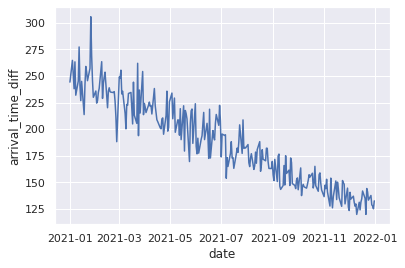
\includegraphics{analise-de-dados/regressao/tempo_chegada_medio.png}
    \caption{Tempo médio de chegada ao longo do Ano}
    \label{fig: tempos_de_chegada}
\end{figure}

A partir dessa percepção, são, então, propostos alguns estudos de regressão mais particulares para representar a tendência dos dados. Um usando "Ordinary Least Squares" e uma regressão exponencial.  

\subsection{Ordinary Least Squares}

Utilizando a biblioteca statsmodel do python foi realizado o estudo de regressão. A Equação Obtida foi: $$intervalos(t) = -0,4933 \cdot t + 252,6629$$. O resumo da regressão e o plot podem ser colocados a seguir: 

\begin{figure}[H]
    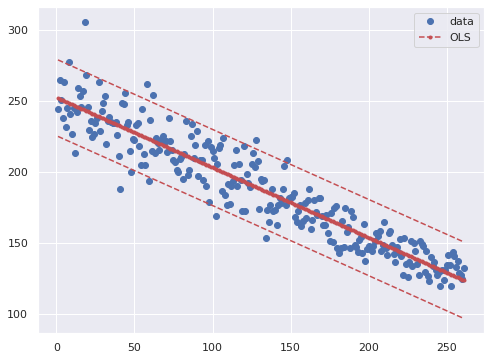
\includegraphics{analise-de-dados/regressao/regressao_OLS.png}
    \caption{Regressão Linear para os tempos de espera}
    \label{fig: plot_OLS}
\end{figure}

\begin{figure}[H]
    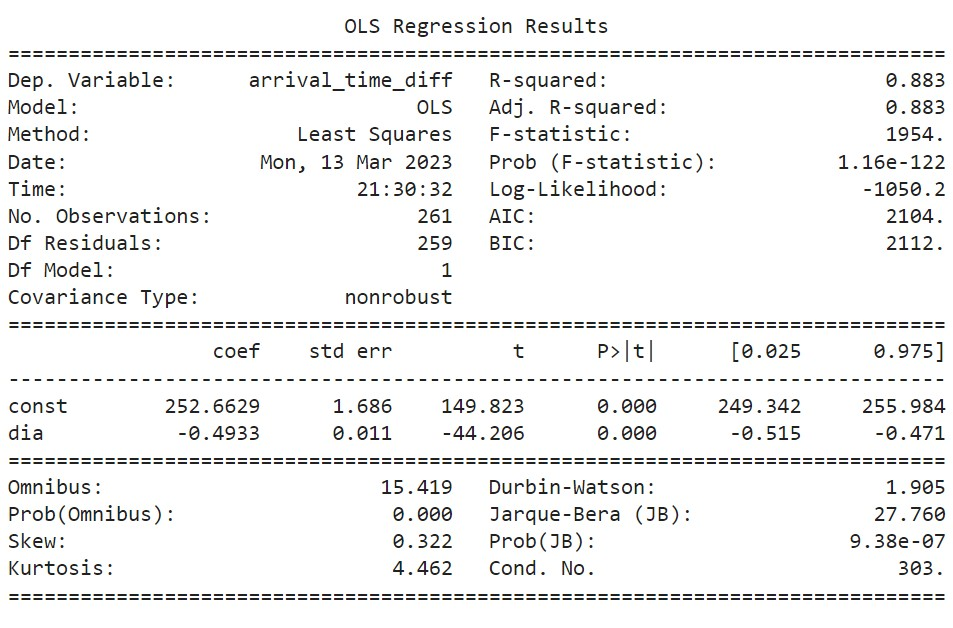
\includegraphics[scale = 0.85]{analise-de-dados/regressao/OLS_summary.jpg}
    \caption{Resumo da regressão}
    \label{fig: sum_OLS}
\end{figure}

Temos que os valores p são menores que o nível de significância adotado, e, portanto, o modelo de regressão existe. Entretanto, para os dias em que $t > 512$ o tempo de chegada das chamadas seria negativo, o que levanta questões sobre se este método de regressão é aplicável para modelar o tempo entre as chamadas.

\subsection{OLS exponencial}

De maneira semelhante ao primeiro estudo, este também foi feito utilizando a biblioteca statsmodel. Entretanto, ao invés dos parâmetros para a regressão terem sido adicionados como são ao modelo, ele foi construído usando: $$ln(y) = ln(b) + a \cdot x$$

Dessa maneira, a equação obtida para representar os dados foi:
$$intervalos(t) = 260,9424 \cdot e^{-0,0027x} $$

O resumo e o gráfico da regressão estão nas imagens 16 e 17:
\begin{figure}[H]
    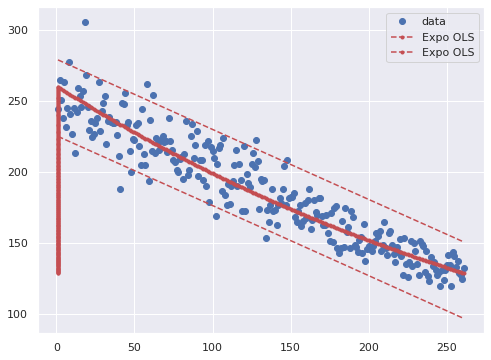
\includegraphics{analise-de-dados/regressao/regressao_EXPO.png}
    \caption{Regressão Exponencial para os tempos de espera}
    \label{fig: plot_Expo_OLS}
\end{figure}

\begin{figure}[H]
    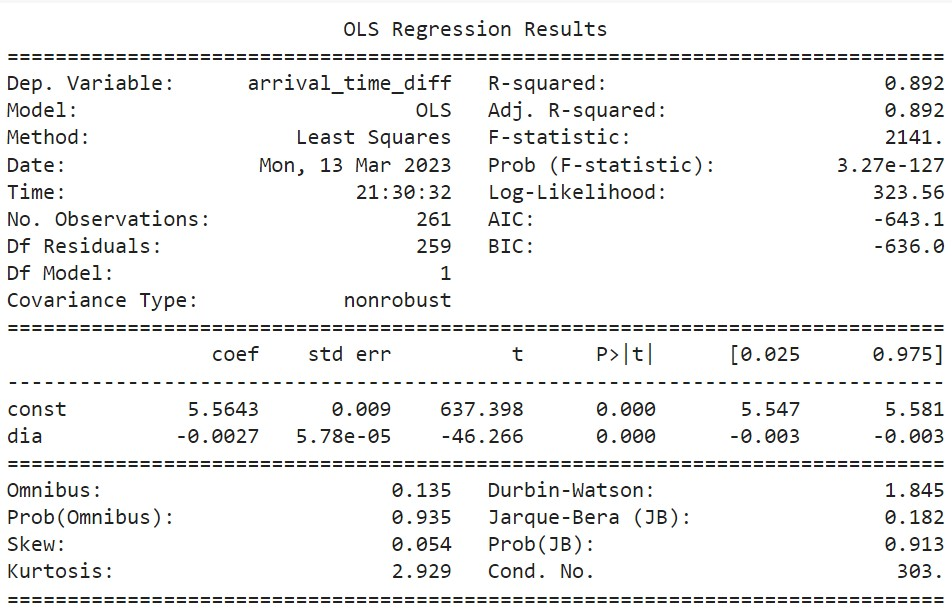
\includegraphics[scale = 0.85]{analise-de-dados/regressao/EXPO_OLS_Summary.jpg}
    \caption{Resumo da regressão}
    \label{fig: sum_Expo_OLS}
\end{figure}

Para Este caso, a explicabilidade do modelo aumentou e o problema que antes existia já não mais existe. Como os Valores P seguem menores do que 0, o modelo existe e pode ser usado.

\subsection{Fit dos tempos entre chegadas para cada mês} 
\label{section: fit-arrivals}
Conforme atestado no teste de hipóteses apresentado na Figura \ref*{fig: ks-arrivals}, o tempo entre as chegadas das ligações muda mês a mês, sendo necessário representar o intervalo entre as chegadas com diferentes distribuições de probabilidade ao longo do tempo em nosso modelo de simulação. A distribuição exponencial é a mais adequada para modelar os dados em todos os meses, visto que apresenta pequenos erros e maiores valores $p$ em relação às demais distribuições.

\subsubsection*{Janeiro}
No primeiro mês do ano, o teste de aderência de Kolgomogorov-Smirnov indica que a distribuição que melhor representa os valores dos tempos entre chegadas é a exponencial com média 248,6240 segundos. A Figura \ref*{fig: fit-janeiro} apresenta o resumo dos testes realizados.

\begin{figure}[H]
    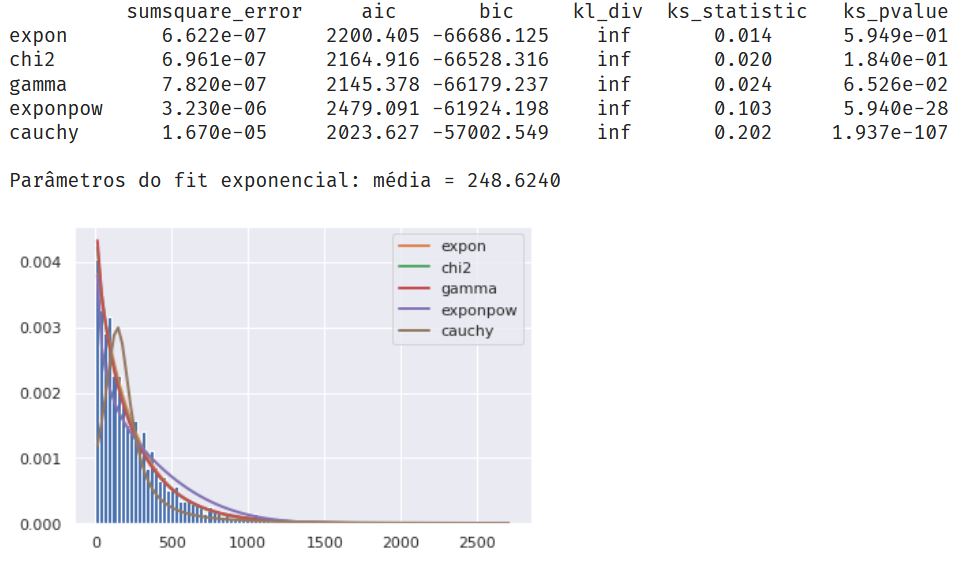
\includegraphics[scale=0.8]{analise-de-dados/fit/fit-janeiro.png}
    \caption{Teste de aderência dos tempos entre chegadas para o mês de janeiro}
    \label{fig: fit-janeiro}
\end{figure}

\subsubsection*{Fevereiro}
No mês de fevereiro, o teste de aderência indica que a distribuição que melhor representa os valores dos tempos entre chegadas é a exponencial com média 231,8853 segundos. A Figura \ref*{fig: fit-fevereiro} apresenta o resumo dos testes realizados.

\begin{figure}[H]
    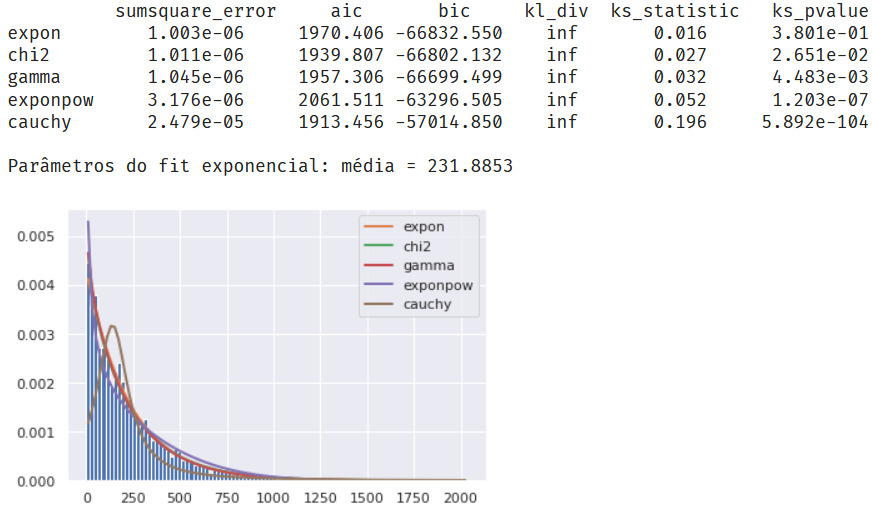
\includegraphics[scale=0.8]{analise-de-dados/fit/fit-fevereiro.png}
    \caption{Teste de aderência dos tempos entre chegadas para o mês de fevereiro}
    \label{fig: fit-fevereiro}
\end{figure}

\subsubsection*{Março}
No mês de março, o teste de aderência indica que a distribuição que melhor representa os valores dos tempos entre chegadas é a exponencial com média 226,2098 segundos. A Figura \ref*{fig: fit-marco} apresenta o resumo dos testes realizados.

\begin{figure}[H]
    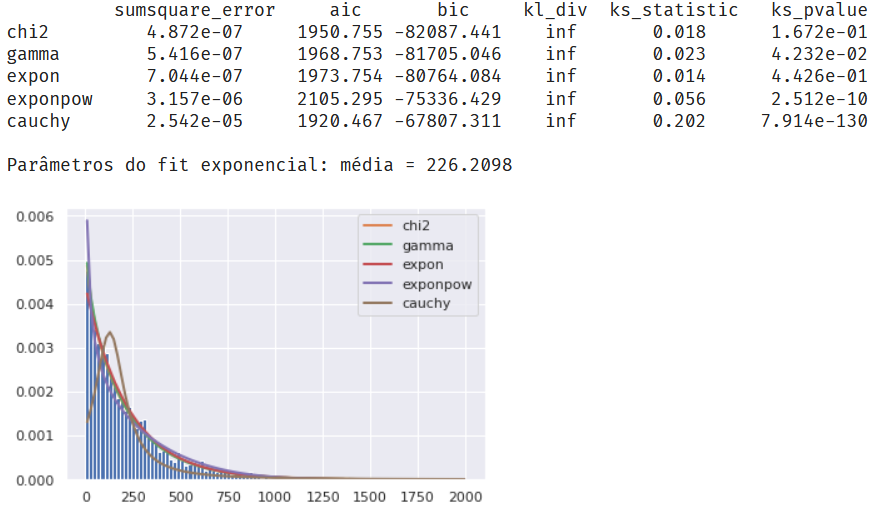
\includegraphics[scale=0.8]{analise-de-dados/fit/fit-marco.png}
    \caption{Teste de aderência dos tempos entre chegadas para o mês de março}
    \label{fig: fit-marco}
\end{figure}

\subsubsection*{Abril}
No mês de abril, o teste de aderência indica que a distribuição que melhor representa os valores dos tempos entre chegadas é a exponencial com média 214,1724 segundos. A Figura \ref*{fig: fit-abril} apresenta o resumo dos testes realizados.

\begin{figure}[H]
    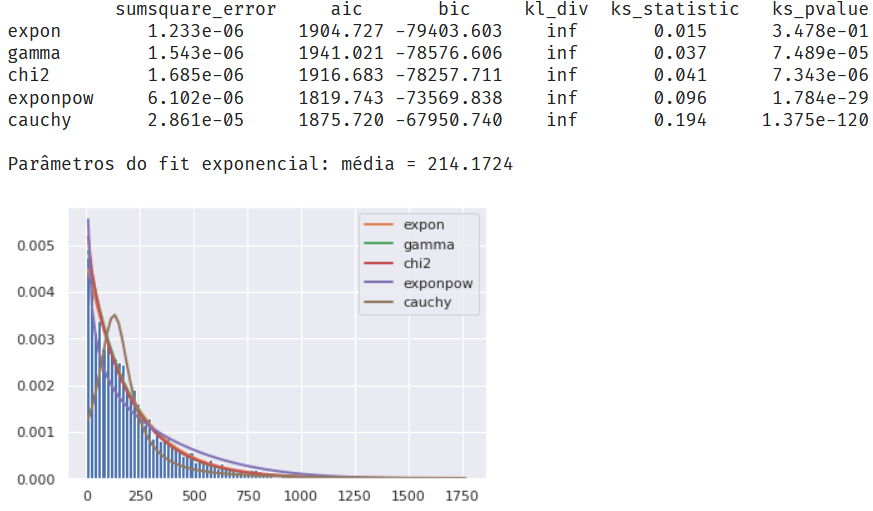
\includegraphics[scale=0.8]{analise-de-dados/fit/fit-abril.png}
    \caption{Teste de aderência dos tempos entre chegadas para o mês de abril}
    \label{fig: fit-abril}
\end{figure}

\subsubsection*{Maio}
No mês de maio, o teste de aderência indica que a distribuição que melhor representa os valores dos tempos entre chegadas é a exponencial com média 206,9737 segundos. A Figura \ref*{fig: fit-maio} apresenta o resumo dos testes realizados.

\begin{figure}[H]
    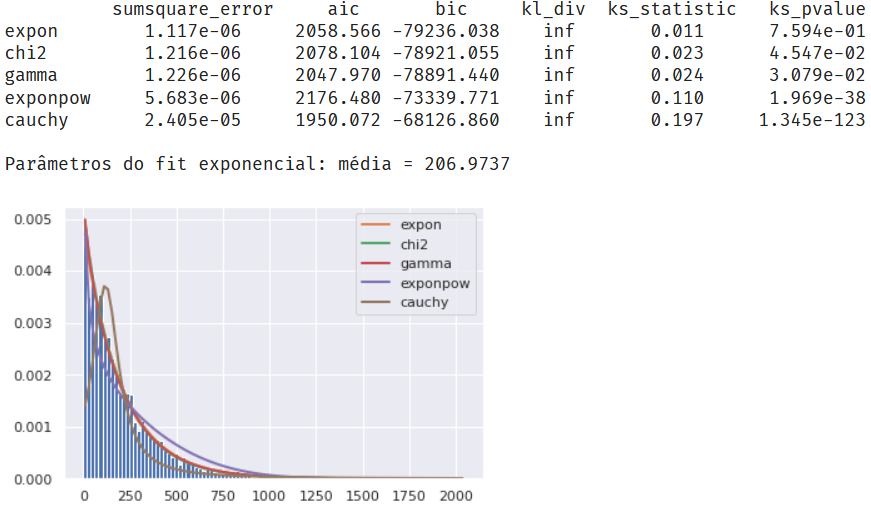
\includegraphics[scale=0.8]{analise-de-dados/fit/fit-maio.png}
    \caption{Teste de aderência dos tempos entre chegadas para o mês de maio}
    \label{fig: fit-maio}
\end{figure}

\subsubsection*{Junho}
No mês de junho, o teste de aderência indica que a distribuição que melhor representa os valores dos tempos entre chegadas é a exponencial com média 195,4312 segundos. A Figura \ref*{fig: fit-junho} apresenta o resumo dos testes realizados.

\begin{figure}[H]
    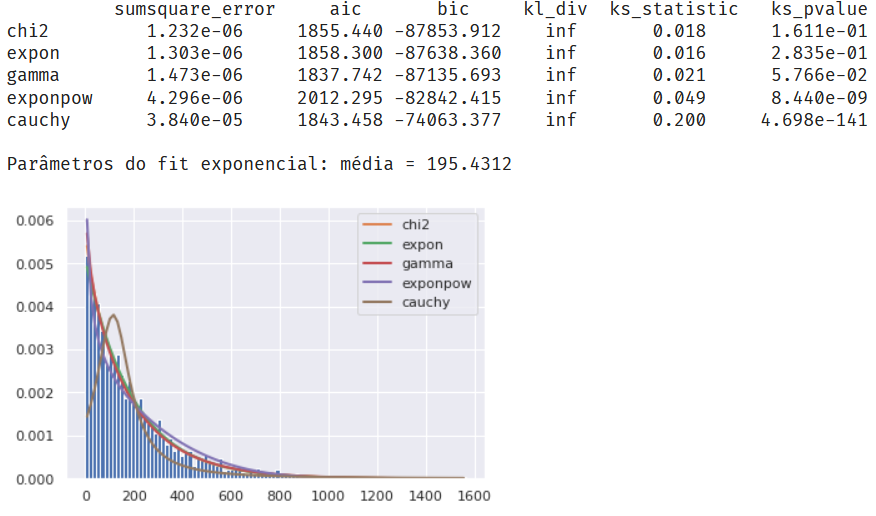
\includegraphics[scale=0.8]{analise-de-dados/fit/fit-junho.png}
    \caption{Teste de aderência dos tempos entre chegadas para o mês de junho}
    \label{fig: fit-junho}
\end{figure}

\subsubsection*{Julho}
No mês de julho, o teste de aderência indica que a distribuição que melhor representa os valores dos tempos entre chegadas é a exponencial com média 180,2765 segundos. A Figura \ref*{fig: fit-julho} apresenta o resumo dos testes realizados.

\begin{figure}[H]
    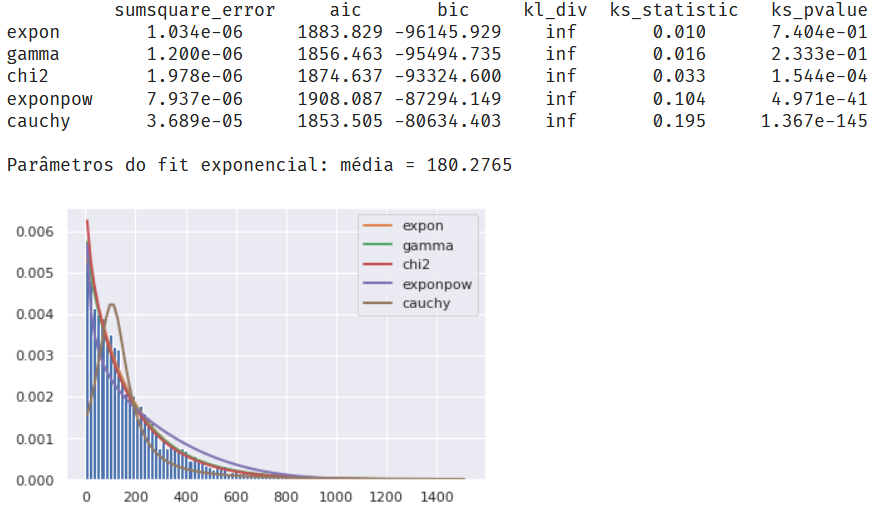
\includegraphics[scale=0.8]{analise-de-dados/fit/fit-julho.png}
    \caption{Teste de aderência dos tempos entre chegadas para o mês de julho}
    \label{fig: fit-julho}
\end{figure}

\subsubsection*{Agosto}
No mês de agosto, o teste de aderência indica que a distribuição que melhor representa os valores dos tempos entre chegadas é a exponencial com média 171,8725 segundos. A Figura \ref*{fig: fit-agosto} apresenta o resumo dos testes realizados.

\begin{figure}[H]
    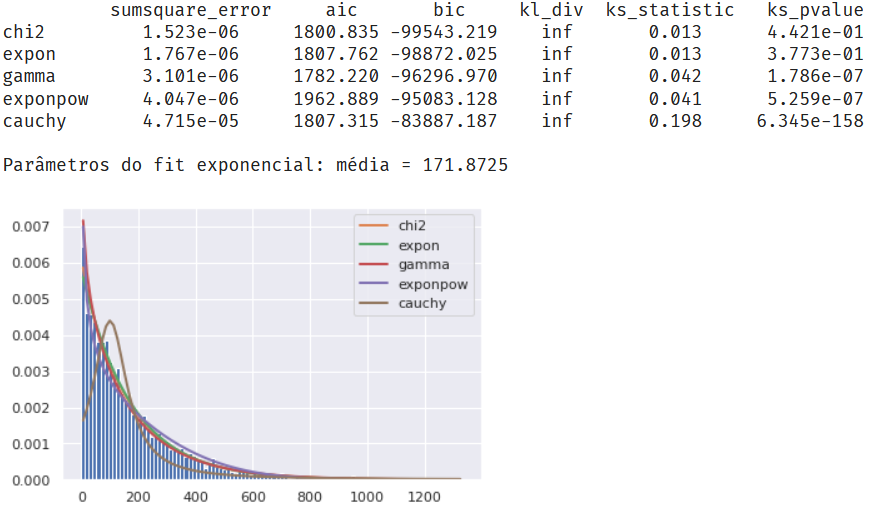
\includegraphics[scale=0.8]{analise-de-dados/fit/fit-agosto.png}
    \caption{Teste de aderência dos tempos entre chegadas para o mês de agosto}
    \label{fig: fit-agosto}
\end{figure}

\subsubsection*{Setembro}
No mês de setembro, o teste de aderência indica que a distribuição que melhor representa os valores dos tempos entre chegadas é a exponencial com média 156,4994 segundos. A Figura \ref*{fig: fit-setembro} apresenta o resumo dos testes realizados.

\begin{figure}[H]
    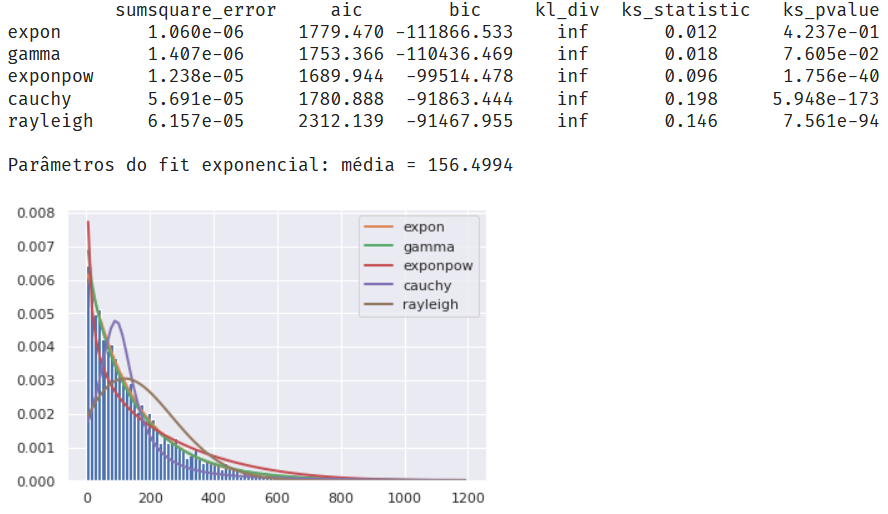
\includegraphics[scale=0.8]{analise-de-dados/fit/fit-setembro.png}
    \caption{Teste de aderência dos tempos entre chegadas para o mês de setembro}
    \label{fig: fit-setembro}
\end{figure}

\subsubsection*{Outubro}
No mês de outubro, o teste de aderência indica que a distribuição que melhor representa os valores dos tempos entre chegadas é a exponencial com média 149,7512 segundos. A Figura \ref*{fig: fit-outubro} apresenta o resumo dos testes realizados.

\begin{figure}[H]
    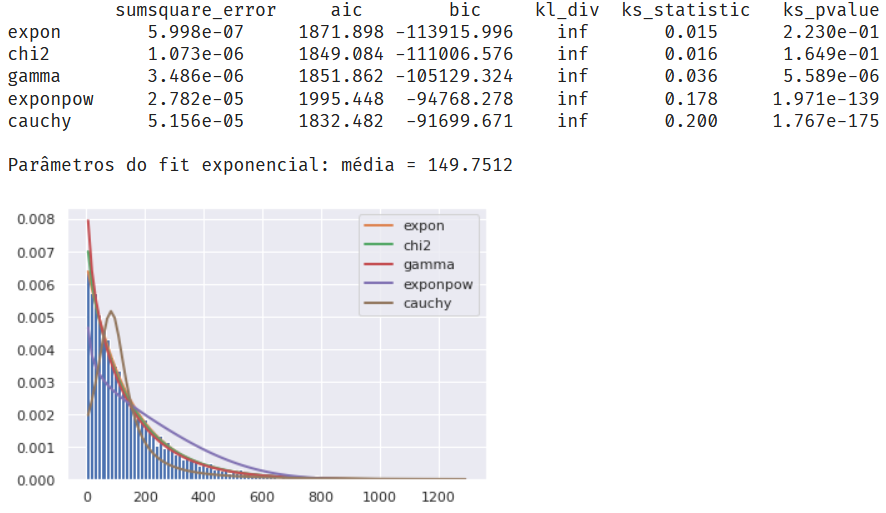
\includegraphics[scale=0.8]{analise-de-dados/fit/fit-outubro.png}
    \caption{Teste de aderência dos tempos entre chegadas para o mês de outubro}
    \label{fig: fit-outubro}
\end{figure}

\subsubsection*{Novembro}
No mês de novembro, o teste de aderência indica que a distribuição que melhor representa os valores dos tempos entre chegadas é a exponencial com média 139,9637 segundos. A Figura \ref*{fig: fit-novembro} apresenta o resumo dos testes realizados.

\begin{figure}[H]
    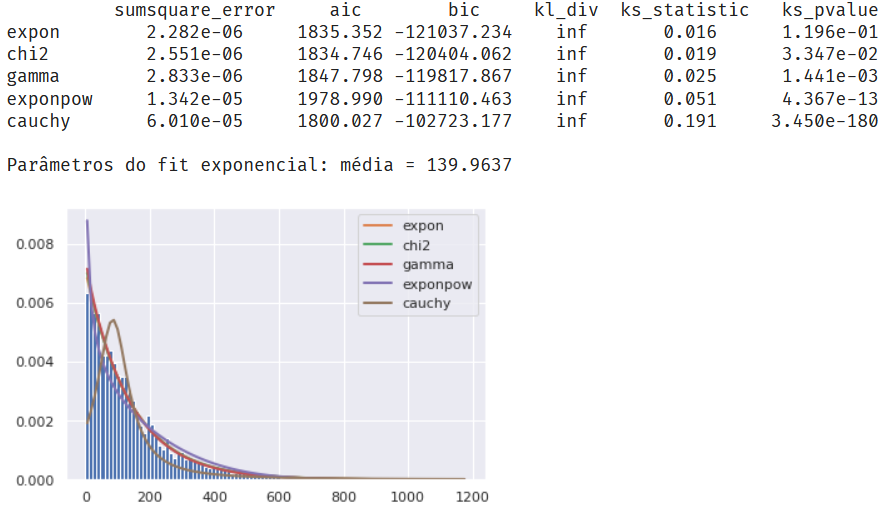
\includegraphics[scale=0.8]{analise-de-dados/fit/fit-novembro.png}
    \caption{Teste de aderência dos tempos entre chegadas para o mês de novembro}
    \label{fig: fit-novembro}
\end{figure}

\subsubsection*{Dezembro}
No mês de dezembro, o teste de aderência indica que a distribuição que melhor representa os valores dos tempos entre chegadas é a exponencial com média 131,3733 segundos. A Figura \ref*{fig: fit-dezembro} apresenta o resumo dos testes realizados.

\begin{figure}[H]
    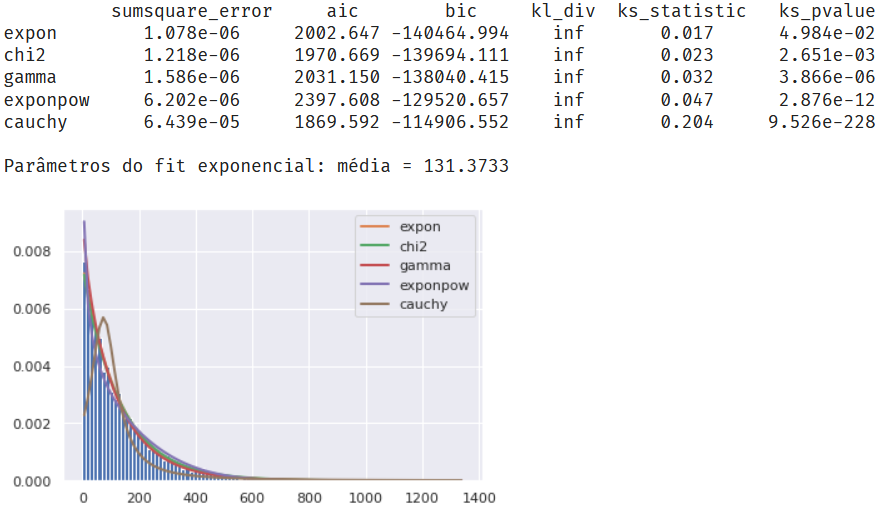
\includegraphics[scale=0.8]{analise-de-dados/fit/fit-dezembro.png}

    \caption{Teste de aderência dos tempos entre chegadas para o mês de dezembro}
    \label{fig: fit-dezembro}
\end{figure}
\subsection{Sumário da análise de dados}
A análise de dados foi um importante processo para o projeto de simulação que está sendo desenvolvido. Por meio dela conseguimos compreender, e testar, quais os melhores níveis de agregação, as distribuições que melhor representam os dados do projeto, o comportamento dos parâmetros e as tendências sob as quais estes se apoiam. Dessa forma, foi possível definir o nível de agregação mensal para o planejamento das atividades do call center, por ser o nível que melhor representa o crescimento do número de chegadas ao longo do ano, assim como modelar os tempos de serviço para o ano inteiro.\\
Restam os esforços para incluir o processo de tendência na simulação e na tomada de decisão para o cliente, garantindo uma assertividade maior ao projeto. Afinal, é esperado que o problema apresentado volte a ocorrer ao longo do tempo se a solução oferecida considerar apenas o estado passado do sistema.

\section{Simulação}
A partir dos dados analisados, foi possível modelar o problema utilizando o software de simulação Arena. A Figura \ref*{fig: ACD} mostra o Diagrama de Ciclo de Atividades (ACD) que auxiliou na modelagem computacional do problema. A Figura \ref*{fig: modelo-arena} apresenta o modelo implementado no Arena. O módulo \textit{Create} nomeado "Chegada"\;recebe uma distribuição de tempo entre chegadas de acordo com os valores modelados na Seção \ref*{section: fit-arrivals}. O módulo \textit{Process} nomeado "Atendimento"\;realiza as ações de \textit{seize}, \textit{delay} e \textit{release} com tempo conforme distribuição exponencial com média 299,1 segundos. São utilizados módulos \textit{Assign} para criar atributos de instante de chegada ("call\_started"), tipo de ligação ("call\_type"), instante de atendimento da chamada ("call\_answered") e instante de fim do atendimento ("call\_ended"). Estes atributos são escritos pelo Arena em um arquivo em formato CSV para posterior análise dos dados.

\begin{figure}[H]
    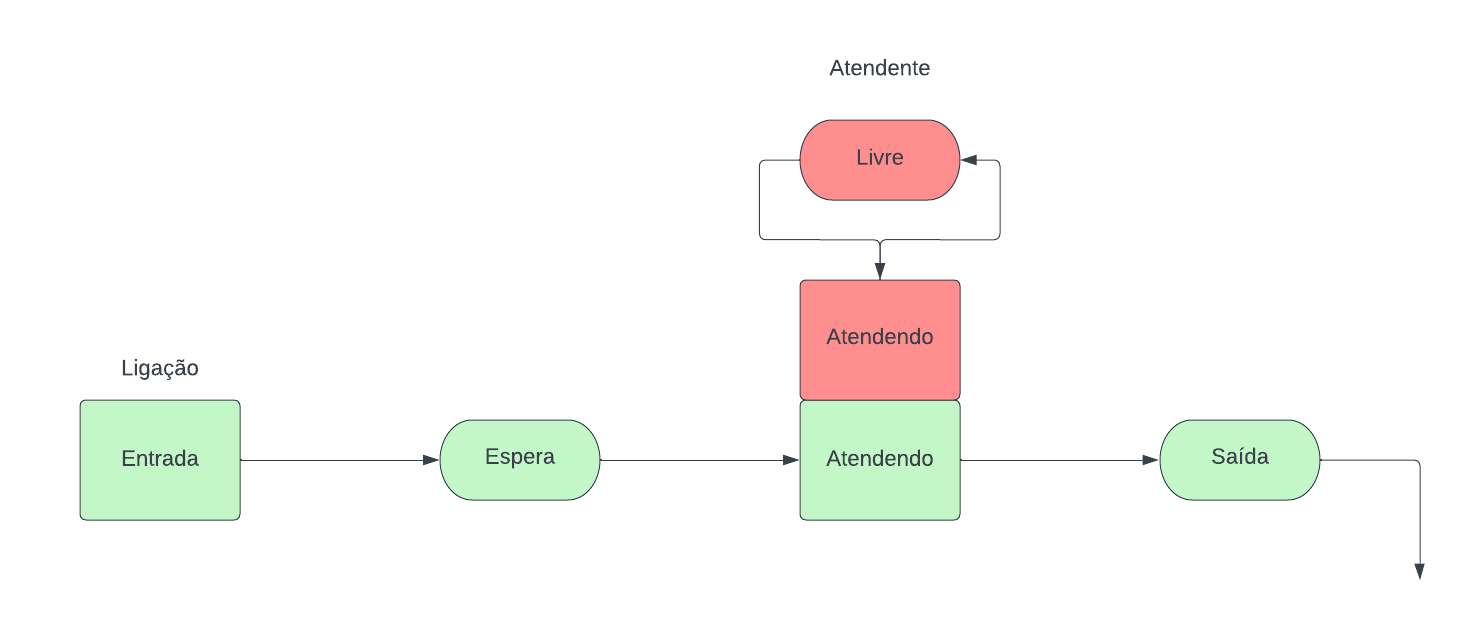
\includegraphics[scale=0.3]{simulacao/acd_vcbc.png}
    \caption{Diagrama de Ciclo de Atividades de uma central de atendimentos}
    \label{fig: ACD}
\end{figure}

\begin{figure}[H]
    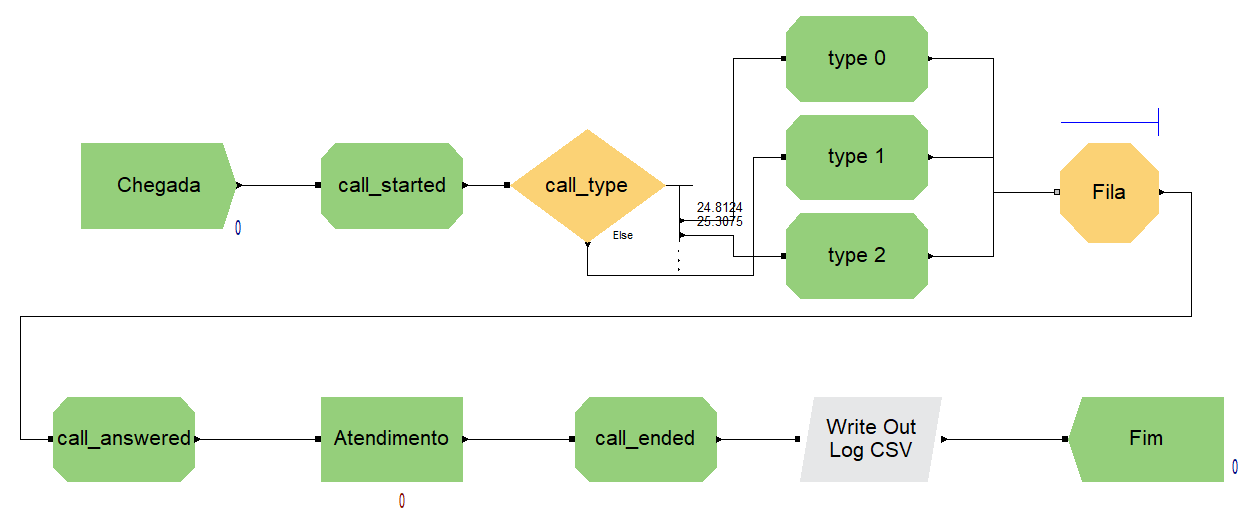
\includegraphics[scale=0.6]{simulacao/modelo-arena.png}
    \caption{Modelo de simulação implementado no Arena}
    \label{fig: modelo-arena}
\end{figure}

A estrutura do arquivo de saída do Arena pode ser vista na Figura \ref*{fig: csv-arena}, após tratamento em Python. Todos os intervalos e instantes registrados estão em segundos.

\begin{figure}[H]
    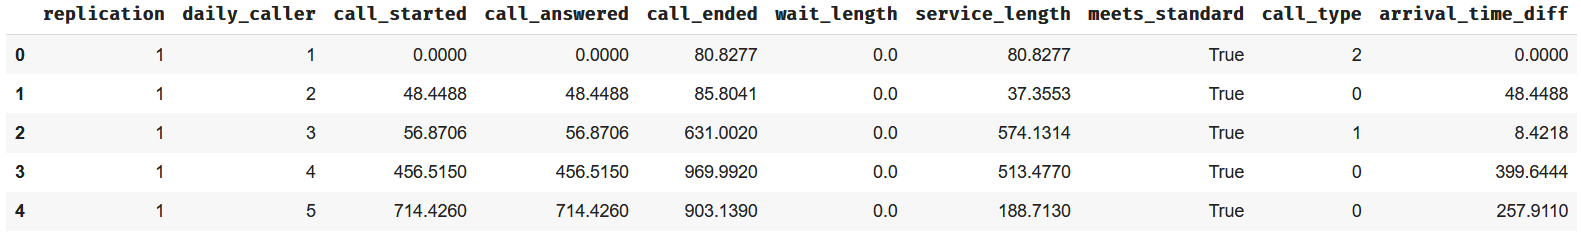
\includegraphics[scale=0.45]{simulacao/csv-arena.png}
    \caption{Primeiras 5 linhas de uma amostra gerada pela simulação no Arena}
    \label{fig: csv-arena}
\end{figure}

\subsection{Validação do modelo}
Para validação do modelo foram realizados testes de hipóteses utilizando o teste de Kolmogorov-Smirnov de 2 amostras para determinar se os valores simulados estão de acordo com os valores históricos. A Tabela \ref*{fig: teste-modelo-historico} apresenta os valores $p$ calculados para cada mês, comparando as amostras dos meses simulados aos valores registrados, assim como o número de replicações aplicado na criação de cada amostra da simulação. Há a rejeição da hipótese nula em três tempos de serviço modelados (valor $p < 0,05$), nos meses de fevereiro, outubro e dezembro.

\begin{table}[H]
    \centering
    \begin{tabular}{|r|r|r|r|r|}
    \hline
     & wait\_length & service\_length & arrival\_time\_diff & Replicações \\ \hline
    Janeiro & 1 & 0,6 & 0,6339 & 21 \\ \hline
    Fevereiro & 1 & \circletext{0,0317} & 0,3055 & 20 \\ \hline
    Março & 1 & 0,6993 & 0,8848 & 23 \\ \hline
    Abril & 0,9898 & 0,09 & 0,1995 & 22 \\ \hline
    Maio & 1 & 0,0869 & 0,5306 & 21 \\ \hline
    Junho & 1 & 0,096 & 0,8442 & 22 \\ \hline
    Julho & 0,9983 & 0,235 & 0,7632 & 22 \\ \hline
    Agosto & 0,4519 & 0,1326 & 0,6323 & 22 \\ \hline
    Setembro & 0,9999 & 0,2445 & 0,8099 & 22 \\ \hline
    Outubro & 0,8217 & \circletext{0,0218} & 0,4198 & 21 \\ \hline
    Novembro & 0,7347 & 0,381 & 0,4229 & 22 \\ \hline
    Dezembro & 0,3517 & \circletext{0,0334} & 0,386 & 23 \\ \hline
    \end{tabular}
    \caption{Valores $p$ dos testes de validação dos tempos do modelo}
    \label{fig: teste-modelo-historico}
\end{table}
    
    
Foi realizado um redimensionamento do número de replicações para tentar compreender a rejeição dos valores obtidos para tempos de serviço. A Tabela \ref*{fig: intervalo-confianca} apresenta, para o mês de dezembro, os intervalos de confiança dos tempos obtidos com 5\% de significância. Para aumentar a precisão dos tempos de serviço, que apresentam maior variância e foram rejeitados no teste de hipótese, foi dimensionado o número de amostras necessárias ($n^*$) para uma precisão desejada ($h^*$) de 3,5 segundos, conforme Tabela \ref*{fig: dimensionamento-corridas}. Como cada replicação deste mês tem em média 270 chamadas, consideramos o valor de 100 replicações para atingir o número de amostras calculado.

\begin{table}[H]
    \begin{tabular}{|l|r|r|r|r|r|r|r|r|r|}
    \hline
    Tempo & \multicolumn{1}{l|}{n} & \multicolumn{1}{l|}{Confiança} & \multicolumn{1}{l|}{$\alpha$} & \multicolumn{1}{l|}{$t$ stat} & \multicolumn{1}{l|}{Desv. Pad.} & \multicolumn{1}{l|}{h} & \multicolumn{1}{l|}{LI} & \multicolumn{1}{l|}{$\mu$} & \multicolumn{1}{l|}{LS} \\ \hline
    Espera & 6213 & 95,00\% & 5,00\% & 1,9603 & 116,0300 & 2,8857 & 39,8890 & 42,7747 & 45,6604 \\ \hline
    Serviço & 6213 & 95,00\% & 5,00\% & 1,9603 & 286,2428 & 7,1190 & 279,8161 & 286,9351 & 294,0540 \\ \hline
    Entre chegadas & 6213 & 95,00\% & 5,00\% & 1,9603 & 134,3537 & 3,3414 & 128,8882 & 132,2297 & 135,5711 \\ \hline
    \end{tabular}
    \caption{Intervalos de confiança das médias dos tempos simulados para o mês de dezembro}
    \label{fig: intervalo-confianca}
\end{table}

\begin{table}[H]
    \centering
    \begin{tabular}{|l|l|l|l|}
    \hline
    n* & n & h & h* \\ \hline
    \multicolumn{1}{|r|}{25703,864} & \multicolumn{1}{r|}{6213} & \multicolumn{1}{r|}{7,1190} & \multicolumn{1}{r|}{3,5} \\ \hline
    \end{tabular}
    \caption{Dimensionamento do número de amostras necessário para maior precisão na validação do modelo}
    \label{fig: dimensionamento-corridas}
\end{table}
    
Executando a validação do modelo com 100 replicações para cada mês, temos na Tabela \ref*{fig: teste-modelo-historico-100} os valores $p$ da comparação das amostras dos meses simulados aos valores históricos, além do percentual médio de falhas em cada mês da simulação, definido como a porcentagem de ligações que levaram mais de 1 minuto para serem atendidas. Neste caso, nenhum $p$ valor ficou abaixo do nível de significância estipulado de 5\%, comprovando que o modelo é bom o suficiente para representar o comportamento dos dados reais em cada um dos meses.

\begin{table}[H]
    \centering
    \begin{tabular}{|l|r|r|r|r|r|}
    \hline
     & \multicolumn{1}{l|}{wait\_length} & \multicolumn{1}{l|}{service\_length} & \multicolumn{1}{l|}{arrival\_time\_diff} & \multicolumn{1}{l|}{Replicações} & \multicolumn{1}{l|}{\% médio de falhas} \\ \hline
    Janeiro & 1 & 0,3175 & 0,311 & 100 & 2,33\% \\ \hline
    Fevereiro & 1 & 0,3135 & 0,0561 & 100 & 2,67\% \\ \hline
    Março & 1 & 0,5948 & 0,685 & 100 & 3,11\% \\ \hline
    Abril & 0,8847 & 0,1727 & 0,0609 & 100 & 3,67\% \\ \hline
    Maio & 1 & 0,561 & 0,3087 & 100 & 4,14\% \\ \hline
    Junho & 1 & 0,4937 & 0,7136 & 100 & 4,73\% \\ \hline
    Julho & 1 & 0,7783 & 0,5795 & 100 & 5,94\% \\ \hline
    Agosto & 0,8023 & 0,6972 & 0,548 & 100 & 7,34\% \\ \hline
    Setembro & 0,971 & 0,8679 & 0,5704 & 100 & 10,27\% \\ \hline
    Outubro & 0,9968 & 0,2854 & 0,8972 & 100 & 11,93\% \\ \hline
    Novembro & 0,148 & 0,7403 & 0,0843 & 100 & 14,59\% \\ \hline
    Dezembro & 0,0719 & 0,6286 & 0,2675 & 100 & 18,17\% \\ \hline
    \end{tabular}
    \caption{Valores $p$ dos testes de validação dos tempos do modelo realizando 100 replicações}
    \label{fig: teste-modelo-historico-100}
\end{table}
    
\subsection{Teste de capacidade da central de atendimentos}
Para avaliar o volume máximo de chamadas que podem ser atendidas sem violar a meta de 90\% das chamadas atendidas em até 1 minuto, isto é, trabalhando com menos de 10\% de falhas, podemos utilizar o modelo de simulação com distribuição dos intervalos entre chegadas próximos do valor modelado para o mês de setembro, no qual o sistema deixa de cumprir a meta, e cuja média do tempo entre chegadas é de 156,4994 segundos. A Tabela \ref{tab: stress-test} apresenta os testes realizados para avaliação da capacidade, executando 100 replicações para cada tempo entre chegadas testado. O volume máximo que pode ser tratado por dia é, em média, 229 chamadas.

\begin{table}[H]
    \centering
    \begin{tabular}{|r|r|r|}
    \hline
    \multicolumn{1}{|l|}{Tempo médio entre chegadas (s)} & \multicolumn{1}{l|}{Quantidade média de chegadas} & \multicolumn{1}{l|}{\% falha} \\ \hline
    160 & 225,14 & 9,64\% \\ \hline
    159 & 226,6 & 9,67\% \\ \hline
    158 & 228,15 & 9,88\% \\ \hline
    157 & 229,59 & 10,11\% \\ \hline
    \end{tabular}
    \caption{Resultados do teste de capacidade da central de atendimento}
    \label{tab: stress-test}
 \end{table}

\section{Conclusão}
\label{section: conclusao}
A análise de dados foi um importante processo para o projeto de simulação que está sendo desenvolvido. Por meio dela conseguimos compreender, e testar, quais os melhores níveis de agregação, as distribuições que melhor representam os dados do projeto, o comportamento dos parâmetros e as tendências sob as quais estes se apoiam. Dessa forma, foi possível definir o nível de agregação mensal para o planejamento das atividades do call center, por ser o nível que melhor representa o crescimento do número de chegadas ao longo do ano, assim como modelar os tempos de serviço para o ano inteiro.

Restam como etapas a modelagem dos processos a serem simulados, bem como dos dados que estes receberão durante a simulação. Em especial, a dos tempos entre chegadas, que são não estacionários e, por consequência, são melhor representados por um processo de Poisson ou algum outro método que leve em consideração o tempo decorrido na simulação. Desta maneira, esse será um dos futuros esforços do projeto.

Outros desses esforços serão incluir o processo de tendência na simulação e na tomada de decisão para o cliente, garantindo uma assertividade maior ao projeto. Afinal, é esperado que o problema apresentado volte a ocorrer no tempo se a solução oferecida apenas resolva o estado presente do sistema.

\end{document}